\section{Nation-State Routing: Default \\Routes}
\label{measure}

As Internet traffic crosses international borders, it becomes subject to the wiretapping policies of the national jurisdiction in which it is transitting.  We study five different countries, Brazil, Netherlands, India, Kenya, and the United States, and measure which countries are transitting their traffic.  The methods we use are described in Section \ref{pipeline1}, and in this section we discuss our findings.

\subsection{Hosting Diversity}
First we look at hosting diversity.  This shows us how many unique countries in which a domain is hosted -- the more countries that a domain is hosted in creates a greater chance that the content is replicated in a favorable country, and could potentially allow a client to circumvent an unfavorable country.  By querying DNS from 26 vantage points around the world, we found that there is hosting diversity among the Alexa Top 100 Domains.  About half of the Alexa Top 100 Domains in each of the five countries studied are hosted in more than one country.  This can be seen in Figure~\ref{fig:host_diversity}.  The amount of hosting diversity motivates the potential for circumventing surveillance states.  We next look at which countries are currently transitting and hosting Internet traffic, and measure whether traffic is going to replicas in surveillance states (when they may not need to).

\begin{figure}
\centering
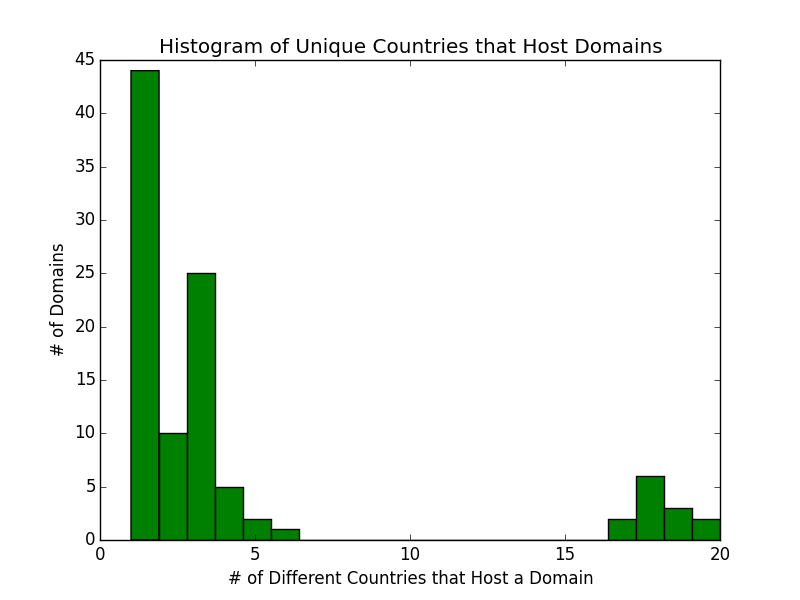
\includegraphics[width=.5\textwidth]{host_domains_hist_US}
\caption{The number of Alexa Top 100 US Domains hosted in different countries.}
\label{fig:host_diversity}
\end{figure}

\subsection{Trend 1: Surveillance States Host Domains}

\newcommand{\headrow}[1]{\multicolumn{1}{c}{\adjustbox{angle=45,lap=\width-0.5em}{#1}}}
\newcommand{\full}{$\bullet$}
\newcommand{\prt}{$\circ$}
\newcolumntype{P}[1]{>{\raggedright\arraybackslash}p{#1}}
%\renewcommand{\familydefault}{\sfdefault}
\noindent
\begin{table*}[h!]
\centering
\begin{tabular}{|P{37mm}|cc|cc|cc|cc|cc|}
\multicolumn{1}{l}{}    & \headrow{Host} & \headrow{Transit} & \headrow{Host} & \headrow{Transit} &\headrow{Host} &\headrow{Transit} &\headrow{Host}   &\headrow{Transit} &\headrow{Host}  &\headrow{Transit} \\\hline
\textit{Country}    &\multicolumn{2}{c|}{\textit{Brazil}}   &\multicolumn{2}{c|}{\textit{Netherlands}}   &\multicolumn{2}{c|}{\textit{India}} &\multicolumn{2}{c|}{\textit{Kenya}} &\multicolumn{2}{c|}{\textit{United States}}\\
\hline\hline
Argentina             &.013     &.013   &     &  &    &   &    &.     &  & \\\hline
Australia             &     &   &     &  &.006    &.047   &.004    &.007     &  & \\\hline
Austria             &    &   &.001     &.015  &    &.001   &    &.002     &  & \\\hline
Bahrain             &     &.00006   &     &  &   &   &    &     &  & \\\hline
Belize             &     &   &     &.0006  &   &.0005   &    &.0006     &  & \\\hline
Brazil             &.169     &1.00   &     &  &   &   &    &     &  & \\\hline
British Virgin Islands  &.001     &.001   &     &  &    &   &    &     &  & \\\hline
Canada             &.001     &.013   &.007     &.007  &.015    &.016   &.006    &.008     &  &.081 \\\hline
Chile             &.00009    &00009   &    & &   &   &   &     &  & \\\hline
China             &     &.0008   &     &.002  &    &.004   &.002    &.003     &  & \\\hline
Costa Rica             &     &   &.009     &.009  &    &  &.002    &.002     &  & \\\hline
Czech Republic             &.002     &.002   &     &.00005  &.001    &.001   &.002    &.002     &  & \\\hline
Denmark             &     &  &     &.0002  &   &   &   &     &  & \\\hline
Finland             &     &   &     &.004  &    &   &    &.003     &  & \\\hline
France             &.001     &.059   &.022     &.102  &.009    &.104   &.023    &.221     &.0013  &.104 \\\hline
Germany             &.002     &.005   &.013     &.050  &.014    &.032   &.028    &.048     &.0013  &.008 \\\hline
Great Britain             &.00006     &.024   &.019     &.140  &.021    &.204   &.032    &.500     &.0024  &.006 \\\hline
Greece             &     &   &     &  &   &  &.003    &.003     &  & \\\hline
Guatemala             &.003     &.003   &     &  &   &   &    &     &  & \\\hline
Hong Kong             &     &   &     &.003  &.004   &.016   &.008   &.012     &  &.0008 \\\hline
India             &    &   &     &.0007  &.053   &1.0   &.002    &.058     &  &.0005 \\\hline
Ireland             &.016     &.028   &.064     &.106  &.027    &.031   &.108    &.133     &.0012  &.006 \\\hline
Israel             &.0001     &.0003   &     &.00005  &.0001    &.002   &.003    &.004     &  & \\\hline
Italy            &.001     &.095   &.008    &.026  &.002    &.008   &.030    &.071     &  &.0003 \\\hline
Japan             &.0003     &.001   &.0001     &.0006  &.001    &.029   &.003    &.016     &.00006  &.00006 \\\hline
Kenya             &    &   &     &  &   &   &.022    &1.0     &  & \\\hline
Latvia             &     &  &.0009     &.0009  &.001    &.001   &.001    &.001     &  & \\\hline
Luxembourg             &    &   &     &.003  &    &   &    &     &  & \\\hline
Malaysia             &     &  &     &  &.003    &.006   &    &     &  & \\\hline
Mauritius             &     &   &     &  &    &   &.004    &.322     &  & \\\hline
Mexico             &     &.0009   &     &  &    &   &    &    &  & \\\hline
Moldova             &     &   &.001     &.001  &.002    &.002   &.002    &.002     &  & \\\hline
Netherlands             &.013     &.019   &.392     &1.0  &.101    &.121   &.200    &.253     &.024  &.031 \\\hline
New Zealand             &    &.003   &     &  &    &   &.003   &.003     &  & \\\hline
Norway             &    &   &.00005     &.001  &    &   &   &     &  & \\\hline
Peru             &     &.00006   &     &  &   &   &   &     &  & \\\hline
Poland             &    &.0002   &     &  &.001    &.012   &   &.0001     &  & \\\hline
Portugal             &    &.0002   &     &  &   &   &.002    &.002     &  & \\\hline
Romania             &     &   &     &.0008  &   &.001   &.002    &.003     &  & \\\hline
Russia             &    &  &     &.00005  &   &   &.005   &.005     &  & \\\hline
Singapore             &    &.0009   &.002     &.002  &.103    &.270   &.027    &.040     &  &.003 \\\hline
South Africa             &    &   &     &  &   &   &.021    &.334     &  & \\\hline
Spain             &.001     &.176   &    &.004  &   &   &   &     &  & \\\hline
Sweden             &.0002     &.001   &.001     &.056  &.003    &.005   &   &.0006     &  &.0003 \\\hline
Switzerland             &     &   &.003     &.004  &.004   &.01   &   &.003     &  & \\\hline
Taiwan             &     &   &     &  &   &  &    &.003     &  & \\\hline
Tanzania             &    &   &     &  &   &   &   &.015     &  & \\\hline
Turkey             &     &   &.003     &.003  &   &   &.003    &.003     &  & \\\hline
Ukraine             &.001     &.001   &     &  &    &   &.002    &.002     &  & \\\hline
United Arab Emirates             &     &.00003   &     &  &   &   &.011    &.152     &  & \\\hline
United States             &.774     &.844   &.454     &.583  &.629    &.715   &.443    &.616     &.969  &1.0 \\\hline
Uruguay             &     &.0003   &    &  &    &   &   &     &  & \\\hline
Venezuela             &    &.003   &     &  &   &   &   &     &  & \\\hline
\end{tabular}
\caption*{}
\label{tab:class}
\end{table*}

\subsection{Trend 2: Traffic Transits Surveillance States}

\subsection{Trend 3: Tromboning Traffic Transits Surveillance States}

\subsection{United States as an Outlier}
